% \section{Jste u nás poprvé?}

% \bigskip
% \subsection{Půjčovna}

% \bigskip
\newcommand\ikonka[1]{\bigskip\bgroup\Large #1\egroup\par}
\ikonka{\faPencil}
\section{Jak se zaregistrovat }

Je to jednoduché a ani kvůli tomu nemusíte osobně navštívit knihovnu.
K~registraci  potřebujete
  průkaz UK (vystavuje na počkání
  \href{http://www.cuni.cz/UK-3249.html}{\emph{Informační a poradenské
  centrum UK}}). Po získání průkazu navštivte stránku \url{knihovna.cuni.cz/e-prihlaska/},
  kde provedete registraci na pouhá dvě kliknutí.

\ikonka{\faBook}
\section{Půjčování a vracení}

Většina knihovního fondu je uložena ve skladu, menší část
v~depozitářích. Ze skladu se půjčuje na počkání, z~depozitářů na
objednávku do dalšího dne nebo k~dohodnutému datu.


Standardní výpůjční lhůta je 30 dní, knihy je možné prodloužit.
K~vracení knih můžete také využít Bibliobox, který se nachází v~přízemí
u vchodu do Pedagogické fakulty a je dostupný po celou dobu provozu
budovy.

\ikonka{\faSearch}
\section{Vše najdete v katalogu nebo~ve~vyhledávači UKAŽ}

Požadované tituly se vyhledávají v~\href{http://ckis.cuni.cz/}{\textbf{Centrálním katalogu UK}}. Každý
dokument je označen signaturou, kterou si zaznamenáte,
a my podle ní knihu vyhledáme. V~katalogu najdete také svůj vlastní
účet, jehož pomocí můžete prodlužovat výpůjčky, rezervovat dokumenty nebo
sledovat stav konta.

\ikonka{\faBed}
\section{Studujte pohodlně z domova}
Kromě papírových knih a časopisů máme i
stovky tisíc textů elektronicky.  V~nabídce jsou elektronické
časopisy, články nebo knihy různých oborů. Jsou dostupné přímo
z~fakultní sítě nebo pomocí vzdáleného přístupu (s využitím
přihlašovacích údajů do Centrální autentizační služby).

Více informací naleznete např. na~\textbf{Portálu elektronických zdrojů
  {\href{https://ezdroje.cuni.cz}{Univerzity Karlovy}}} nebo ve \textbf{vyhledávači UKAŽ}.



% \newpage

\ikonka{\faGraduationCap}
\section{Vyzkoušejte naši studovnu}

% Pro prezenční studium dokumentů je určena studovna knihovny. 
% Tu mohou využívat studenti s~platným průkazem UK, ale i externí uživatelé. 
% Uloženy jsou zde 
Ve studovně najdete odborné knihy, odborné i populárně naučné
časopisy, učebnice, skripta a vždy aktuální denní tisk.

Využít můžete také počítače s přístupem na~internet a do databází,
samoobslužné tiskárny, kopírky a skener. Nabízíme také vázání kroužkovou vazbou.

% Můžete využít i doplňkových služeb a vypůjčit si 
Půjčujeme i notebooky, USB nabíječky na
telefon, čtečky elektronických knih, deskové hry nebo flash disky (vše
v~rámci studovny).

\textbf{Máme pro vás také týmovou studovnu.} Rezervovat si ji můžete
vyplněním formuláře na~našem webu. V týmové studovně je k dispozici deset míst
a tabule na~psaní.

% \subsection{Další služby a nástroje}

% \newpage


\ikonka{\faAndroid}
\section{Pomoc s citacemi}

Tvořit citace je jednoduché: nechte za sebe pracovat citační manažer.
Pokud studujete nebo pracujete na~Pedagogické fakultě,
můžete bezplatně využívat citační manažer Citace PRO.
Pokud si s citacemi nevíte rady, rádi pomůžeme.

\bigskip
\ikonka{\faHeart}
\section{Služby pro studenty se~speciálními potřebami}

Připravili jsme pro vás počítač s~asistenčním softwarem
a~možností tisku a~kopírování zdarma. Pro studenty se zrakovými obtížemi
nabízíme přístup ke knihám v~elektronické podobě a~kamerovou
zvětšovací lupu. 
Vítáni jsou také čtenáři s pohybovým hendikepem.  
\newpage
\section{Kde nás najdete?}

\vskip 3em
\smallsection{Půjčovna a studovna v hlavní budově fakulty}

% Těšíme se na~vás v přízemí hlavní budovy Pedagogické fakulty
% na~adrese 
Magdaleny Rettigové 4, Praha 1\\
v přízemí, nalevo od vrátnice.

\vskip 3em
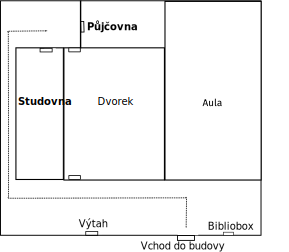
\includegraphics[width=\textwidth]{svgplanek.pdf}

\vskip 4em
\smallsection{Studovna jazyků v Celetné}

Celetná 13, Praha 1, 4. patro


% \textbf{Jak se k~nám dostanete?}

% \begin{itemize}[leftmargin=0pt, topsep=0pt]
% \item
%   metrem B, stanice Národní třída -- výtahem přímo do ulice Magdalény
%   Rettigové
% \item
%   tramvají č. 3, 6, 9, 14, 24 zastávka Lazarská
% \end{itemize}

% \smallsection{Knihovna je rozdělena na dvě části:}

% \begin{itemize}[leftmargin=0pt, topsep=0pt]
% \item Půjčovna se nachází napravo od hlavního vchodu
%   do budovy, přes dvorek, vedle zadního vchodu do Auly.
% \item Studovna  je na levé straně budovy.
% \end{itemize}

  % \rotatebox{90}{% Graphic for TeX using PGF
% Title: /home/mint/knihovna/planekknihovny.dia
% Creator: Dia v0.97.3
% CreationDate: Tue Oct 10 14:49:24 2017
% For: mint
% \usepackage{tikz}
% The following commands are not supported in PSTricks at present
% We define them conditionally, so when they are implemented,
% this pgf file will use them.
\ifx\du\undefined
  \newlength{\du}
\fi
\setlength{\du}{11\unitlength}
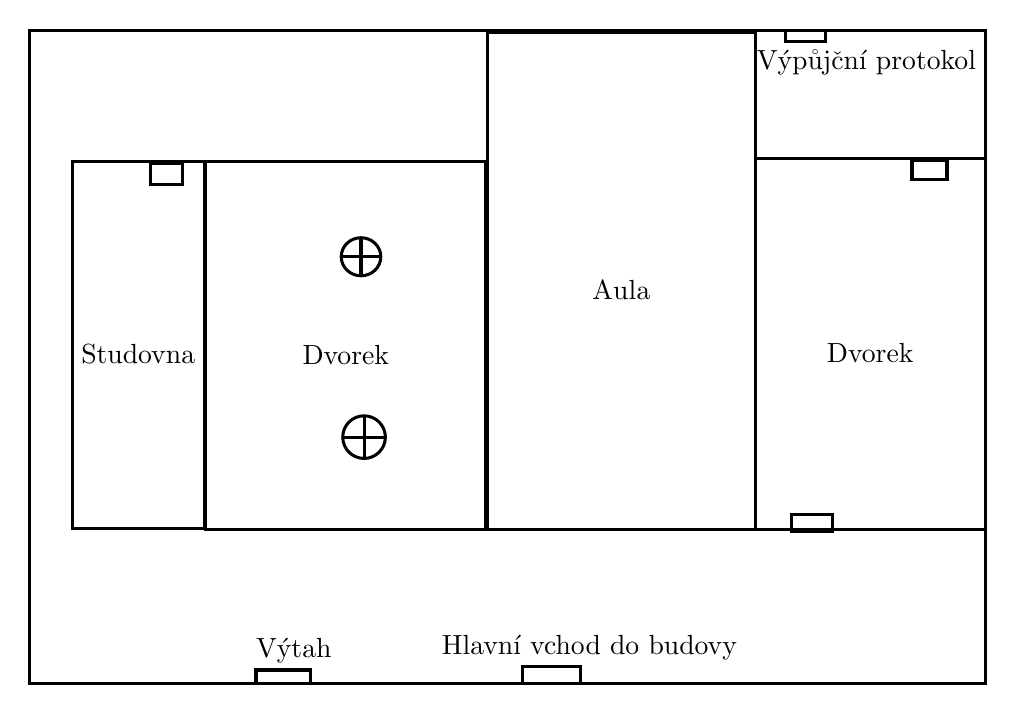
\begin{tikzpicture}
\pgftransformxscale{1.000000}
\pgftransformyscale{-1.000000}
\definecolor{dialinecolor}{rgb}{0.000000, 0.000000, 0.000000}
\pgfsetstrokecolor{dialinecolor}
\definecolor{dialinecolor}{rgb}{1.000000, 1.000000, 1.000000}
\pgfsetfillcolor{dialinecolor}
\definecolor{dialinecolor}{rgb}{1.000000, 1.000000, 1.000000}
\pgfsetfillcolor{dialinecolor}
\fill (0.300000\du,4.300000\du)--(0.300000\du,25.750000\du)--(31.700000\du,25.750000\du)--(31.700000\du,4.300000\du)--cycle;
\pgfsetlinewidth{0.100000\du}
\pgfsetdash{}{0pt}
\pgfsetdash{}{0pt}
\pgfsetmiterjoin
\definecolor{dialinecolor}{rgb}{0.000000, 0.000000, 0.000000}
\pgfsetstrokecolor{dialinecolor}
\draw (0.300000\du,4.300000\du)--(0.300000\du,25.750000\du)--(31.700000\du,25.750000\du)--(31.700000\du,4.300000\du)--cycle;
% setfont left to latex
\definecolor{dialinecolor}{rgb}{0.000000, 0.000000, 0.000000}
\pgfsetstrokecolor{dialinecolor}
\node at (16.000000\du,15.310000\du){};
\definecolor{dialinecolor}{rgb}{1.000000, 1.000000, 1.000000}
\pgfsetfillcolor{dialinecolor}
\fill (6.100000\du,8.600000\du)--(6.100000\du,20.700000\du)--(15.300000\du,20.700000\du)--(15.300000\du,8.600000\du)--cycle;
\pgfsetlinewidth{0.100000\du}
\pgfsetdash{}{0pt}
\pgfsetdash{}{0pt}
\pgfsetmiterjoin
\definecolor{dialinecolor}{rgb}{0.000000, 0.000000, 0.000000}
\pgfsetstrokecolor{dialinecolor}
\draw (6.100000\du,8.600000\du)--(6.100000\du,20.700000\du)--(15.300000\du,20.700000\du)--(15.300000\du,8.600000\du)--cycle;
% setfont left to latex
\definecolor{dialinecolor}{rgb}{0.000000, 0.000000, 0.000000}
\pgfsetstrokecolor{dialinecolor}
\node at (10.700000\du,14.935000\du){Dvorek};
\definecolor{dialinecolor}{rgb}{1.000000, 1.000000, 1.000000}
\pgfsetfillcolor{dialinecolor}
\fill (15.350000\du,4.350000\du)--(15.350000\du,20.700000\du)--(24.150000\du,20.700000\du)--(24.150000\du,4.350000\du)--cycle;
\pgfsetlinewidth{0.100000\du}
\pgfsetdash{}{0pt}
\pgfsetdash{}{0pt}
\pgfsetmiterjoin
\definecolor{dialinecolor}{rgb}{0.000000, 0.000000, 0.000000}
\pgfsetstrokecolor{dialinecolor}
\draw (15.350000\du,4.350000\du)--(15.350000\du,20.700000\du)--(24.150000\du,20.700000\du)--(24.150000\du,4.350000\du)--cycle;
% setfont left to latex
\definecolor{dialinecolor}{rgb}{0.000000, 0.000000, 0.000000}
\pgfsetstrokecolor{dialinecolor}
\node at (19.750000\du,12.810000\du){Aula};
\pgfsetlinewidth{0.100000\du}
\pgfsetdash{}{0pt}
\pgfsetdash{}{0pt}
\pgfsetbuttcap
\pgfsetmiterjoin
\pgfsetlinewidth{0.100000\du}
\pgfsetbuttcap
\pgfsetmiterjoin
\pgfsetdash{}{0pt}
\definecolor{dialinecolor}{rgb}{1.000000, 1.000000, 1.000000}
\pgfsetfillcolor{dialinecolor}
\pgfpathellipse{\pgfpoint{11.300000\du}{17.650000\du}}{\pgfpoint{0.700000\du}{0\du}}{\pgfpoint{0\du}{0.700000\du}}
\pgfusepath{fill}
\definecolor{dialinecolor}{rgb}{0.000000, 0.000000, 0.000000}
\pgfsetstrokecolor{dialinecolor}
\pgfpathellipse{\pgfpoint{11.300000\du}{17.650000\du}}{\pgfpoint{0.700000\du}{0\du}}{\pgfpoint{0\du}{0.700000\du}}
\pgfusepath{stroke}
\pgfsetbuttcap
\pgfsetmiterjoin
\pgfsetdash{}{0pt}
\definecolor{dialinecolor}{rgb}{0.000000, 0.000000, 0.000000}
\pgfsetstrokecolor{dialinecolor}
\draw (11.300000\du,16.950000\du)--(11.300000\du,18.350000\du);
\pgfsetbuttcap
\pgfsetmiterjoin
\pgfsetdash{}{0pt}
\definecolor{dialinecolor}{rgb}{0.000000, 0.000000, 0.000000}
\pgfsetstrokecolor{dialinecolor}
\draw (10.600000\du,17.650000\du)--(12.000000\du,17.650000\du);
\pgfsetlinewidth{0.100000\du}
\pgfsetdash{}{0pt}
\pgfsetdash{}{0pt}
\pgfsetbuttcap
\pgfsetmiterjoin
\pgfsetlinewidth{0.100000\du}
\pgfsetbuttcap
\pgfsetmiterjoin
\pgfsetdash{}{0pt}
\definecolor{dialinecolor}{rgb}{1.000000, 1.000000, 1.000000}
\pgfsetfillcolor{dialinecolor}
\pgfpathellipse{\pgfpoint{11.200000\du}{11.725000\du}}{\pgfpoint{0.650000\du}{0\du}}{\pgfpoint{0\du}{0.625000\du}}
\pgfusepath{fill}
\definecolor{dialinecolor}{rgb}{0.000000, 0.000000, 0.000000}
\pgfsetstrokecolor{dialinecolor}
\pgfpathellipse{\pgfpoint{11.200000\du}{11.725000\du}}{\pgfpoint{0.650000\du}{0\du}}{\pgfpoint{0\du}{0.625000\du}}
\pgfusepath{stroke}
\pgfsetbuttcap
\pgfsetmiterjoin
\pgfsetdash{}{0pt}
\definecolor{dialinecolor}{rgb}{0.000000, 0.000000, 0.000000}
\pgfsetstrokecolor{dialinecolor}
\draw (11.200000\du,11.100000\du)--(11.200000\du,12.350000\du);
\pgfsetbuttcap
\pgfsetmiterjoin
\pgfsetdash{}{0pt}
\definecolor{dialinecolor}{rgb}{0.000000, 0.000000, 0.000000}
\pgfsetstrokecolor{dialinecolor}
\draw (10.550000\du,11.725000\du)--(11.850000\du,11.725000\du);
\definecolor{dialinecolor}{rgb}{1.000000, 1.000000, 1.000000}
\pgfsetfillcolor{dialinecolor}
\fill (24.153750\du,8.500000\du)--(24.153750\du,20.700000\du)--(31.700000\du,20.700000\du)--(31.700000\du,8.500000\du)--cycle;
\pgfsetlinewidth{0.100000\du}
\pgfsetdash{}{0pt}
\pgfsetdash{}{0pt}
\pgfsetmiterjoin
\definecolor{dialinecolor}{rgb}{0.000000, 0.000000, 0.000000}
\pgfsetstrokecolor{dialinecolor}
\draw (24.153750\du,8.500000\du)--(24.153750\du,20.700000\du)--(31.700000\du,20.700000\du)--(31.700000\du,8.500000\du)--cycle;
% setfont left to latex
\definecolor{dialinecolor}{rgb}{0.000000, 0.000000, 0.000000}
\pgfsetstrokecolor{dialinecolor}
\node at (27.926875\du,14.885000\du){Dvorek};
\definecolor{dialinecolor}{rgb}{1.000000, 1.000000, 1.000000}
\pgfsetfillcolor{dialinecolor}
\fill (1.707500\du,8.600000\du)--(1.707500\du,20.650000\du)--(6.050000\du,20.650000\du)--(6.050000\du,8.600000\du)--cycle;
\pgfsetlinewidth{0.100000\du}
\pgfsetdash{}{0pt}
\pgfsetdash{}{0pt}
\pgfsetmiterjoin
\definecolor{dialinecolor}{rgb}{0.000000, 0.000000, 0.000000}
\pgfsetstrokecolor{dialinecolor}
\draw (1.707500\du,8.600000\du)--(1.707500\du,20.650000\du)--(6.050000\du,20.650000\du)--(6.050000\du,8.600000\du)--cycle;
% setfont left to latex
\definecolor{dialinecolor}{rgb}{0.000000, 0.000000, 0.000000}
\pgfsetstrokecolor{dialinecolor}
\node at (3.878750\du,14.910000\du){Studovna};
\pgfsetlinewidth{0.100000\du}
\pgfsetdash{}{0pt}
\pgfsetdash{}{0pt}
\pgfsetmiterjoin
\definecolor{dialinecolor}{rgb}{1.000000, 1.000000, 1.000000}
\pgfsetfillcolor{dialinecolor}
\fill (25.350000\du,20.200000\du)--(25.350000\du,20.350000\du)--(26.700000\du,20.350000\du)--(26.700000\du,20.200000\du)--cycle;
\definecolor{dialinecolor}{rgb}{0.000000, 0.000000, 0.000000}
\pgfsetstrokecolor{dialinecolor}
\draw (25.350000\du,20.200000\du)--(25.350000\du,20.750000\du)--(26.700000\du,20.750000\du)--(26.700000\du,20.200000\du)--cycle;
\pgfsetlinewidth{0.100000\du}
\pgfsetdash{}{0pt}
\pgfsetdash{}{0pt}
\pgfsetmiterjoin
\definecolor{dialinecolor}{rgb}{1.000000, 1.000000, 1.000000}
\pgfsetfillcolor{dialinecolor}
\fill (29.300000\du,8.550000\du)--(29.300000\du,9.200000\du)--(30.450000\du,9.200000\du)--(30.450000\du,8.550000\du)--cycle;
\definecolor{dialinecolor}{rgb}{0.000000, 0.000000, 0.000000}
\pgfsetstrokecolor{dialinecolor}
\draw (29.300000\du,8.550000\du)--(29.300000\du,9.200000\du)--(30.450000\du,9.200000\du)--(30.450000\du,8.550000\du)--cycle;
\pgfsetlinewidth{0.100000\du}
\pgfsetdash{}{0pt}
\pgfsetdash{}{0pt}
\pgfsetmiterjoin
\definecolor{dialinecolor}{rgb}{1.000000, 1.000000, 1.000000}
\pgfsetfillcolor{dialinecolor}
\fill (25.150000\du,4.200000\du)--(25.150000\du,4.650000\du)--(26.450000\du,4.650000\du)--(26.450000\du,4.200000\du)--cycle;
\definecolor{dialinecolor}{rgb}{0.000000, 0.000000, 0.000000}
\pgfsetstrokecolor{dialinecolor}
\draw (25.150000\du,4.300000\du)--(25.150000\du,4.650000\du)--(26.450000\du,4.650000\du)--(26.450000\du,4.300000\du)--cycle;
\pgfsetlinewidth{0.100000\du}
\pgfsetdash{}{0pt}
\pgfsetdash{}{0pt}
\pgfsetmiterjoin
\definecolor{dialinecolor}{rgb}{1.000000, 1.000000, 1.000000}
\pgfsetfillcolor{dialinecolor}
\fill (4.300000\du,8.650000\du)--(4.300000\du,9.350000\du)--(5.350000\du,9.350000\du)--(5.350000\du,8.650000\du)--cycle;
\definecolor{dialinecolor}{rgb}{0.000000, 0.000000, 0.000000}
\pgfsetstrokecolor{dialinecolor}
\draw (4.300000\du,8.650000\du)--(4.300000\du,9.350000\du)--(5.350000\du,9.350000\du)--(5.350000\du,8.650000\du)--cycle;
\pgfsetlinewidth{0.100000\du}
\pgfsetdash{}{0pt}
\pgfsetdash{}{0pt}
\pgfsetmiterjoin
\definecolor{dialinecolor}{rgb}{1.000000, 1.000000, 1.000000}
\pgfsetfillcolor{dialinecolor}
\fill (16.500000\du,25.200000\du)--(16.500000\du,25.750000\du)--(18.400000\du,25.750000\du)--(18.400000\du,25.200000\du)--cycle;
\definecolor{dialinecolor}{rgb}{0.000000, 0.000000, 0.000000}
\pgfsetstrokecolor{dialinecolor}
\draw (16.500000\du,25.200000\du)--(16.500000\du,25.750000\du)--(18.400000\du,25.750000\du)--(18.400000\du,25.200000\du)--cycle;
% setfont left to latex
\definecolor{dialinecolor}{rgb}{0.000000, 0.000000, 0.000000}
\pgfsetstrokecolor{dialinecolor}
\node[anchor=west] at (16.000000\du,15.025000\du){};
% setfont left to latex
\definecolor{dialinecolor}{rgb}{0.000000, 0.000000, 0.000000}
\pgfsetstrokecolor{dialinecolor}
\node[anchor=west] at (23.850000\du,5.350000\du){Výpůjční protokol};
% setfont left to latex
\definecolor{dialinecolor}{rgb}{0.000000, 0.000000, 0.000000}
\pgfsetstrokecolor{dialinecolor}
\node[anchor=west] at (13.500000\du,24.550000\du){Hlavní vchod do budovy};
\pgfsetlinewidth{0.100000\du}
\pgfsetdash{}{0pt}
\pgfsetdash{}{0pt}
\pgfsetmiterjoin
\definecolor{dialinecolor}{rgb}{1.000000, 1.000000, 1.000000}
\pgfsetfillcolor{dialinecolor}
\fill (7.750000\du,25.300000\du)--(7.750000\du,25.650000\du)--(9.550000\du,25.650000\du)--(9.550000\du,25.300000\du)--cycle;
\definecolor{dialinecolor}{rgb}{0.000000, 0.000000, 0.000000}
\pgfsetstrokecolor{dialinecolor}
\draw (7.750000\du,25.300000\du)--(7.750000\du,25.750000\du)--(9.550000\du,25.750000\du)--(9.550000\du,25.300000\du)--cycle;
% setfont left to latex
\definecolor{dialinecolor}{rgb}{0.000000, 0.000000, 0.000000}
\pgfsetstrokecolor{dialinecolor}
\node[anchor=west] at (7.400000\du,24.650000\du){Výtah};
\end{tikzpicture}
}

\newpage
\section{Kontakty}

\begin{tabular}{@{}ll@{}}
  E-mail:& \url{knihovna@pedf.cuni.cz}\\

  Půjčovna& 221\,900\,148\\
  Studovna:& 221\,900\,178\\
  Studovna Celetná:& 221\,900\,759\\
  Facebook: & \url{@knihovnapedfpraha}\\
  Instagram: & \url{@knihovnapedfpraha}
\end{tabular}

  % \newpage
\section{Otevírací doba}

\noindent\smallsection{Půjčovna v M. Rettigové}

\ifdefined\HCode
\begin{tabular}{lllll}
  Po      & ~ & 8.00 &--& 16.00\\
  Út--pá  & ~ & 8.00 &--& 17.00
\end{tabular}

\else
\begin{tabular}{@{}ll}
  Po--Pá & 9.00 -- 17.00\\
\end{tabular}

\fi

\vskip 2em
\noindent\smallsection{Studovna v M. Rettigové}

\begin{tabular}{@{}ll}
  Po--Čt &  8.00 -- 18.00\\
  Pá     &  8.00 -- 17.00\\
\end{tabular}

\vskip 2em
\noindent\smallsection{Studovna v Celetné}

\begin{tabular}{@{}ll}
  Út\phantom{--Pá} &  13.00 -- 18.45\\
  Čt &  10.00 -- 14.00\\
  Pá & 13.00 -- 17.45\\
\end{tabular}
\vskip 2em
\section{Odkazy}

\footnotesize
\begin{tabular}{@{}ll@{}}
  Knihovna PedF UK:& \url{knihovna.pedf.cuni.cz} \\

  Centrální katalog UK:& \url{ckis.cuni.cz} \\

  Centrální autentizační služba:& \url{cas.cuni.cz}\\

  Portál elektronických zdrojů:& \url{ezdroje.cuni.cz}\\

  Vyhledávač UKAŽ:& \url{ukaz.cuni.cz} \\

  Citace PRO: & \url{citace.com/citace-pro} \\

  % Ústřední knihovna UK:& \url{knihovna.cuni.cz} \\

  % IPSC UK:& \url{ipc.cuni.cz} 
\end{tabular}
% \newpage
